
\subsection{Fotodioden}
Photodioden sind beleuchtete pn-Übergänge. Im Kurzschlussbetrieb (U = 0) fließt ein über einen Bereich von mehr als acht Zehnerpotenzen linear von der Beleuchtungsstärke abhängiger Kurzschlussstrom $I_k$ (Abbildung \ref{fig:PhotodiodeKennline})
\cite{Aktive_Bauelemente}.
Dieser setzt sich aus dem durch einstrahlendes Licht verursachten Photostrom und dem temperaturabhängen Dunkelstrom Zusammen \cite{Halbleiterelektronik}.
Allerdings hängt der Photostrom auch von der Absorptionstiefe in das Siliziumsubstrat ab, welche wiederum von der Wellenlänge abhängt (Abbildung  \ref{fig:Silizium-eindingtiefe}) \cite{osiopto_electronics}

\begin{figure}[H]
  \begin{subfigure}[b]{0.4\textwidth}
  \caption{Kennlinienfeld Photodiode \cite{Aktive_Bauelemente}}
    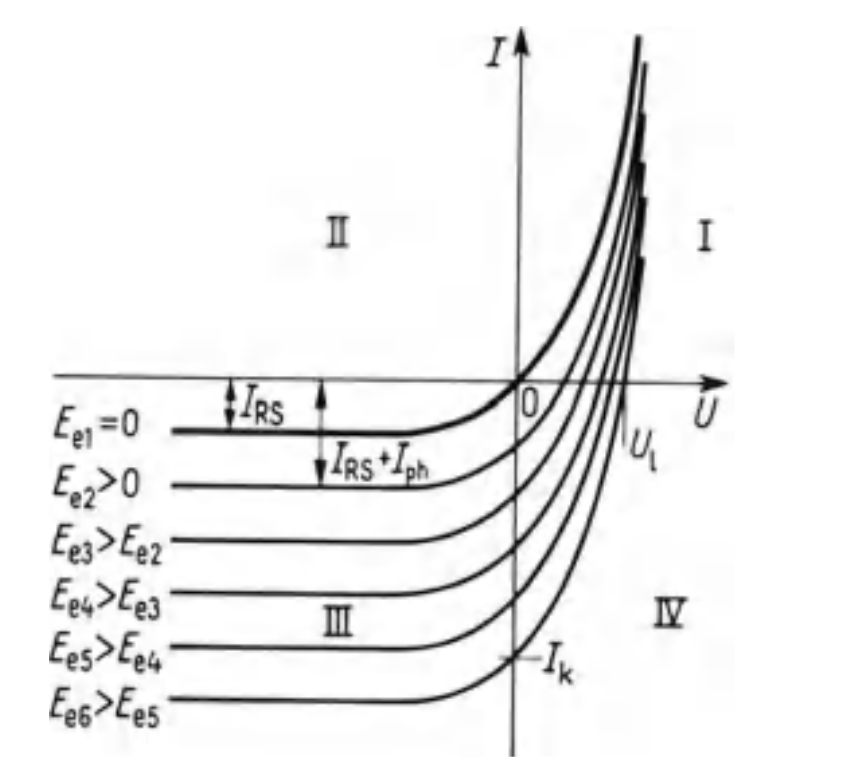
\includegraphics[width=\textwidth]{img/Photodiode-Kennline.png}
    \caption*{Kennlinienfeld $I=f(U)$ der \\Photodiode mit der Bestrah-\\lungsstärke $E_e$ als Parameter\\Kurzschlussstrom $I_k$ bei $U=0$}
    \label{fig:PhotodiodeKennline}
  \end{subfigure}
  %
  \begin{subfigure}[b]{0.55\textwidth}
    \caption{Silizium-Eindringtiefe-Licht \cite{laser}}
    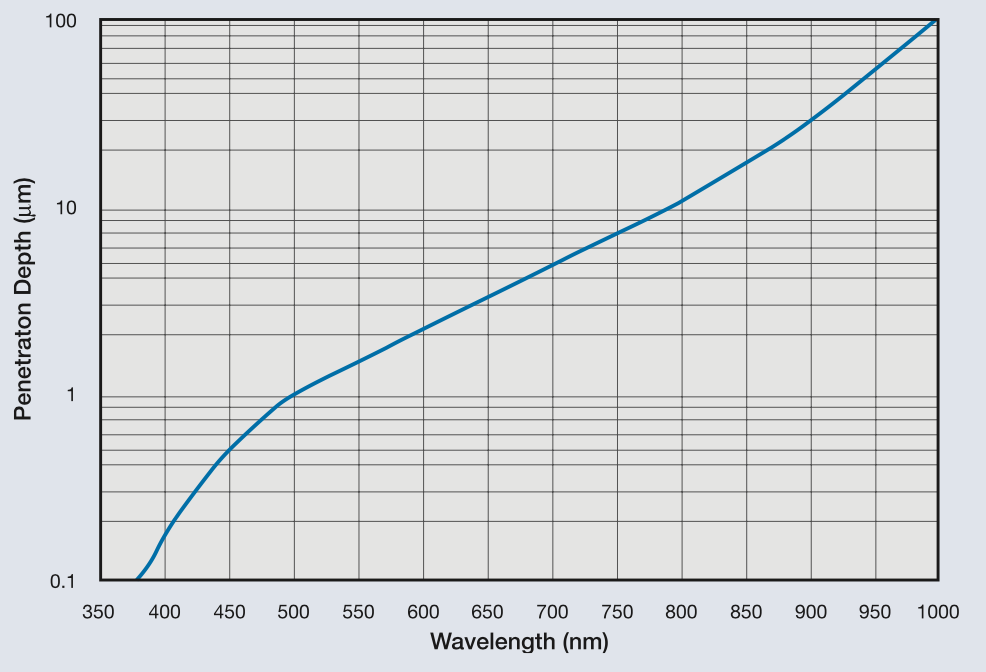
\includegraphics[width=\textwidth]{img/Silizium-Eindringtiefe-Licht.png}
    \caption*{ Optische Eigenschaften von Silizium: Absorptionskoeffizient (Dreiecke) und Absorptionstiefe (Kreise) in Abhängigkeit von der Wellenlänge.}
  \label{fig:Silizium-eindingtiefe}
  \end{subfigure}
\end{figure}







\noindent Damit Rückschlüsse über den Kurzschlussstrom $I_K$ zur Lichtintensität zulässig sind, muss also die Temperatur konstant oder zumindest bekannt sein, da so ein möglichst akkurater temperatur- und frequenzabhängiger Kompensationsfaktor gewählt werden kann.
%\subsection{Analog Digital Wanlder}
\subsection{I2C}
I2C ist ein simples und effizientes Busprotokoll.
Es wurde ursprünglich von Phillips entwickelt, wird aber seit einigen Jahren von NPX weiterentwickelt.
In seiner simpelsten Form ermöglicht es einen Master mit bis zu 128 Slave-Geräten zu verbinden.
Dafür werden nur 2 Leitungen benötigt, die SCL und SDA genannt werden. SCL ist die Taktleitung. Sie wird verwendet, um alle Datenübertragungen über den I2C-Bus zu synchronisieren. SDA ist die Datenleitung.
Alle Busteilnehmer müssen mit dem gleichen GND potential verbunden sein um Stromfluss über die SDA und SCL Leitungen zu ermöglichen\cite{i2b-bus_org}.\\
SCL und SDA benötigen jeweils einen Pull-Up-Widerstand da sie als ”Open Drain” betrieben werden, was bedeutet, dass die Leitungen über Widerstände (Pull-Up-Widerstände) mit der Versorgungsspannung verbunden sind und somit in den High-Zustand gezogen werden.
Die angeschlossenen Geräte ändern den Zustand der Datenleitung auf Low, indem sie die Leitung über einen MOSFET mit GND verbinden.
Um die Leitung wieder auf High zu heben, wird die Verbindung zu GND wieder getrennt und der Pull-Up-Widerstand sorgt dafür, dass die Leitung wieder im High-Zustand ist.\\
Die Clockleitung SCL wird vom Bus Master gesteuert, so kann der Master den Takt der Datenübertragung bestimmen.
Die SDA Leitung wird vom Master und Slave genutzt um Daten zu übertragen. Allerdings antworten die Slaves im Normalbetrieb nur, nachdem sie vom Master auf iher Adresse eine Anfrage erhalten haben. 
Die Spezifikation des Protokolls\cite{nxp_com} empfiehlt die SDA und SCL Leitung möglichst weit voneinander zu entfernen um so Signalstörungen vorzubeugen.


